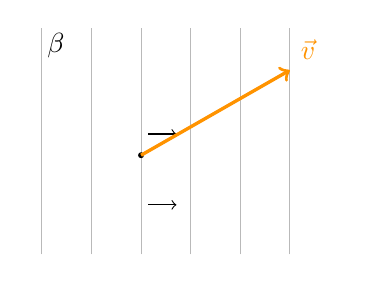
\begin{tikzpicture}[scale=0.9]
  % beta: vertical family of lines
  \clip (-2.2,-1.6) rectangle (2.2,1.6);
  \foreach \x in {-2,-1.3,...,2} {
    \draw[gray!55, line width=0.35pt] (\x,-1.6) -- (\x,1.6);
  }
  % direction markers
  \draw[->, black, line width=0.4pt] (-0.5,-0.9) -- (-0.1,-0.9);
  \draw[->, black, line width=0.4pt] (-0.5,0.1) -- (-0.1,0.1);

  % vector v
  \fill[black] (-0.6,-0.2) circle (1.2pt);
  \draw[->, very thick, orange!85!yellow] (-0.6,-0.2) -- (1.5,1.0) node[above right] {$\vec{v}$};

  \node at (-1.8,1.35) {$\beta$};
\end{tikzpicture}
